\section{Story Patterns (Christian und Marie)} \label{sec:StoryPatterns}

\todoch{Define concrete syntax for new elements. In particular, check syntax for links.}


\subsection{Story Pattern [CH]}

general idea, purpose, attributes (matching, normal)

\subsection{Objects and Object Variables [MCP]}

%Object variables represent the objects defined in a story pattern.
%They are identified by their name.
%The objects are instances of classes of the underlying classmodel (cp. Section \ref{typedGraphTransformations}).
%Thus, the object variables are typed by classes from this model.

%\begin{figure}[htbp]
%\begin{center}
%  \includegraphics[width=0.25\textwidth]{figures/objectVariable}
%  \caption{An object variable}
%  \label{fig:objectVariable}
%\end{center}
%\end{figure}
%Figure \ref{fig:objectVariable} shows an object variable with the name \texttt{methodDecl} and the type
%\texttt{Method}.

\todomcp{Are Primitive Variables part of this section? Should we have an own Section dealing with them?}

\todomcp{What is the concrete syntax for primitive variables? How do we assign values to them?}

\todomcp{Are primitive variables connected to other nodes in the story pattern? What is their scope/lifetime? Do they exist beyond the end of the Activity?}

\subsection{Links and Link Variables [MCP]}

\subsection{Binding of Variables [MCP]}

%Object variables and link variables have binding operators, binding states, and binding semantics.

\subsubsection{Binding Operators}
%The binding operators define whether an element is to be created, deleted, or just matched.
%After all elements that are defined to be deleted or just matched have been matched, the model ist modified by creating
%and deleting the elements as defined. 

%Elements to be created are marked with the
%label \texttt{CREATE} and elements to be deleted are marked with the label \texttt{DESTROY}.

\subsubsection{Binding States}

\subsubsection{Binding Semantics}

\todomcp{Negative objects, Figure \ref{fig:negativeObjects}:
a) allowed; same semantics for the same situation with link not negative
b) not allowed because graph is not connected
c) allowed?
d) allowed because a and b are both bound
e) not allowed
f) allowed; same semantics for the same situation with links not negative
}

\begin{figure}[htbp]
  \centering
  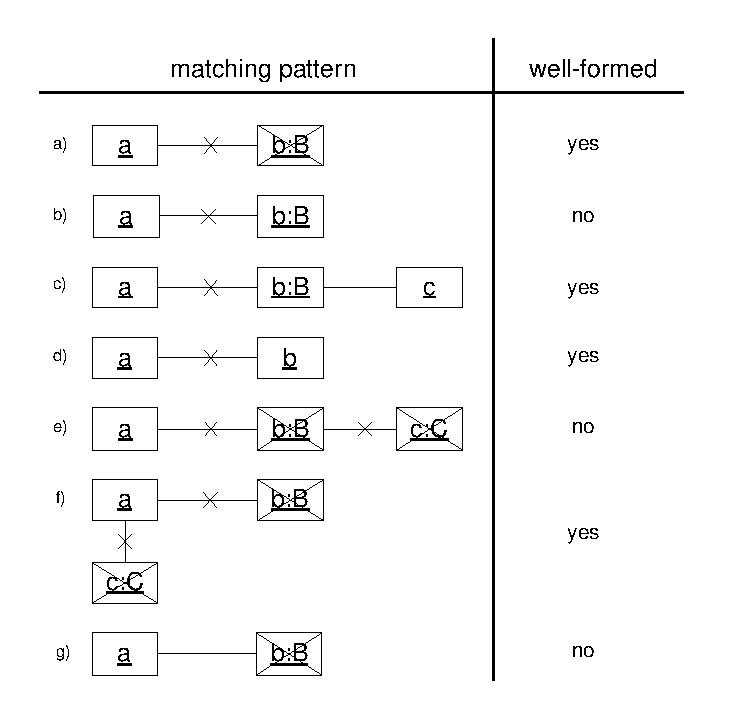
\includegraphics[scale=1]{figures/negativeObjects}
  \caption{Negative Objects}
  \label{fig:negativeObjects}
\end{figure}

\todomcp{Optional objects, Figure \ref{fig:optionalObjects}:
the same as for negative objects?
a) allowed; same semantics for the same situation with link not optional?
b) not allowed because graph is not connected
c) allowed?
d) allowed because a and b are both bound
e) not allowed
f) allowed; same semantics for the same situation with links not optional
}

\begin{figure}[htbp]
  \centering
  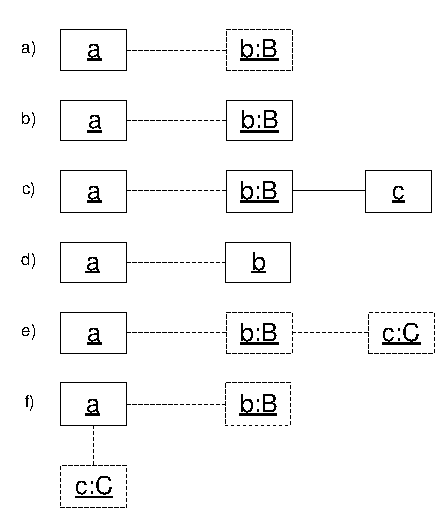
\includegraphics[scale=1]{figures/optionalObjects}
  \caption{Optional Objects}
  \label{fig:optionalObjects}
\end{figure}


\subsubsection{Feasible Binding Combinations}

\todomcp{check Table \ref{tab:bindingCombinations}}
% Table generated by Excel2LaTeX from sheet 'Tabelle1'
\begin{table}[htbp]
  \centering
  \caption{Feasible combinations of binding operators, binding states, and binding semantics}
    \begin{tabular}{|r|r|r|r|}
    \hline
    \textbf{Binding Operator} & \textbf{Binding State} & \textbf{Binding Semantics} & \textbf{Result} \\
    \hline
    CHECK\_ONLY & UNBOUND & MANDATORY & yes \\
    CHECK\_ONLY & UNBOUND & NEGATIVE & yes \\
    CHECK\_ONLY & UNBOUND & OPTIONAL & yes \\
    CHECK\_ONLY & BOUND & MANDATORY & yes \\
    CHECK\_ONLY & BOUND & NEGATIVE & no \\
    CHECK\_ONLY & BOUND & OPTIONAL & no \\
    CHECK\_ONLY & MAYBE\_BOUND & MANDATORY & yes \\
    CHECK\_ONLY & MAYBE\_BOUND & NEGATIVE & no \\
    CHECK\_ONLY & MAYBE\_BOUND & OPTIONAL & no \\
    \hline
    CREATE & UNBOUND & MANDATORY & yes \\
    CREATE & UNBOUND & NEGATIVE & no \\
    CREATE & UNBOUND & OPTIONAL & yes \\
    CREATE & BOUND & MANDATORY & no \\
    CREATE & BOUND & NEGATIVE & no \\
    CREATE & BOUND & OPTIONAL & no \\
    CREATE & MAYBE\_BOUND & MANDATORY & no \\
    CREATE & MAYBE\_BOUND & NEGATIVE & no \\
    CREATE & MAYBE\_BOUND & OPTIONAL & no \\
    \hline
    DESTROY & UNBOUND & MANDATORY & yes \\
    DESTROY & UNBOUND & NEGATIVE & no \\
    DESTROY & UNBOUND & OPTIONAL & yes \\
    DESTROY & BOUND & MANDATORY & yes \\
    DESTROY & BOUND & NEGATIVE & no \\
    DESTROY & BOUND & OPTIONAL & no \\
    DESTROY & MAYBE\_BOUND & MANDATORY & yes \\
    DESTROY & MAYBE\_BOUND & NEGATIVE & no \\
    DESTROY & MAYBE\_BOUND & OPTIONAL & no \\
    \hline
    \end{tabular}%
  \label{tab:bindingCombinations}%
\end{table}%


\subsection{Using Object Attributes [CH]}

object constraints, attribute assignments

\subsection{Object Sets [MCP]}

explain objectSetVariables, set size expressions

\todomcp{object sets and binding operators/states/semantics}

\todomcp{If we bind an object set, can we use the bound object in other story pattern? E.g. to insert all elements bound by the object set into a container via a containment link? (See Figure \ref{fig:reuseObjSet}).}

\begin{figure}[htbp]
  \centering
  
\includegraphics[scale=1.0]{figures/ReuseObjectSet}
  \caption{Reusing Object Sets}
  \label{fig:reuseObjSet}
\end{figure}

\todomcp{What happens if an object set contains no ObjectSetSizeExpression and no object is matched into the object set? Proposal: ObjectSet is interpreted as optional and the matching succeeds.}

\todomcp{What happens if $\leq$ is used in the ObjectSetSizeExpression and there exist more objects in the graph that could be matched into the set? E.g., the pattern in Figure \ref{fig:objSetSize} is applied to a class with 3 methods. Is  $\leq$ allowed as an operator in this case? Proposal: The operator is allowed and the pattern does not match.}

\begin{figure}[htbp]
  \centering
  
\includegraphics[scale=1.0]{figures/ObjectSetSize}
  \caption{Object Set Size}
  \label{fig:objSetSize}
\end{figure}

\todomcp{What happens if one pattern contains two object sets that may possibly contain the same objects. Consider the pattern in Figure \ref{fig:isoObjSet}. If c1 and c2 share the same super classes, su1 and su2 contain the same objects. Is this allowed? Isomorphic matching would normally forbid this.}

\begin{figure}[htbp]
  \centering
  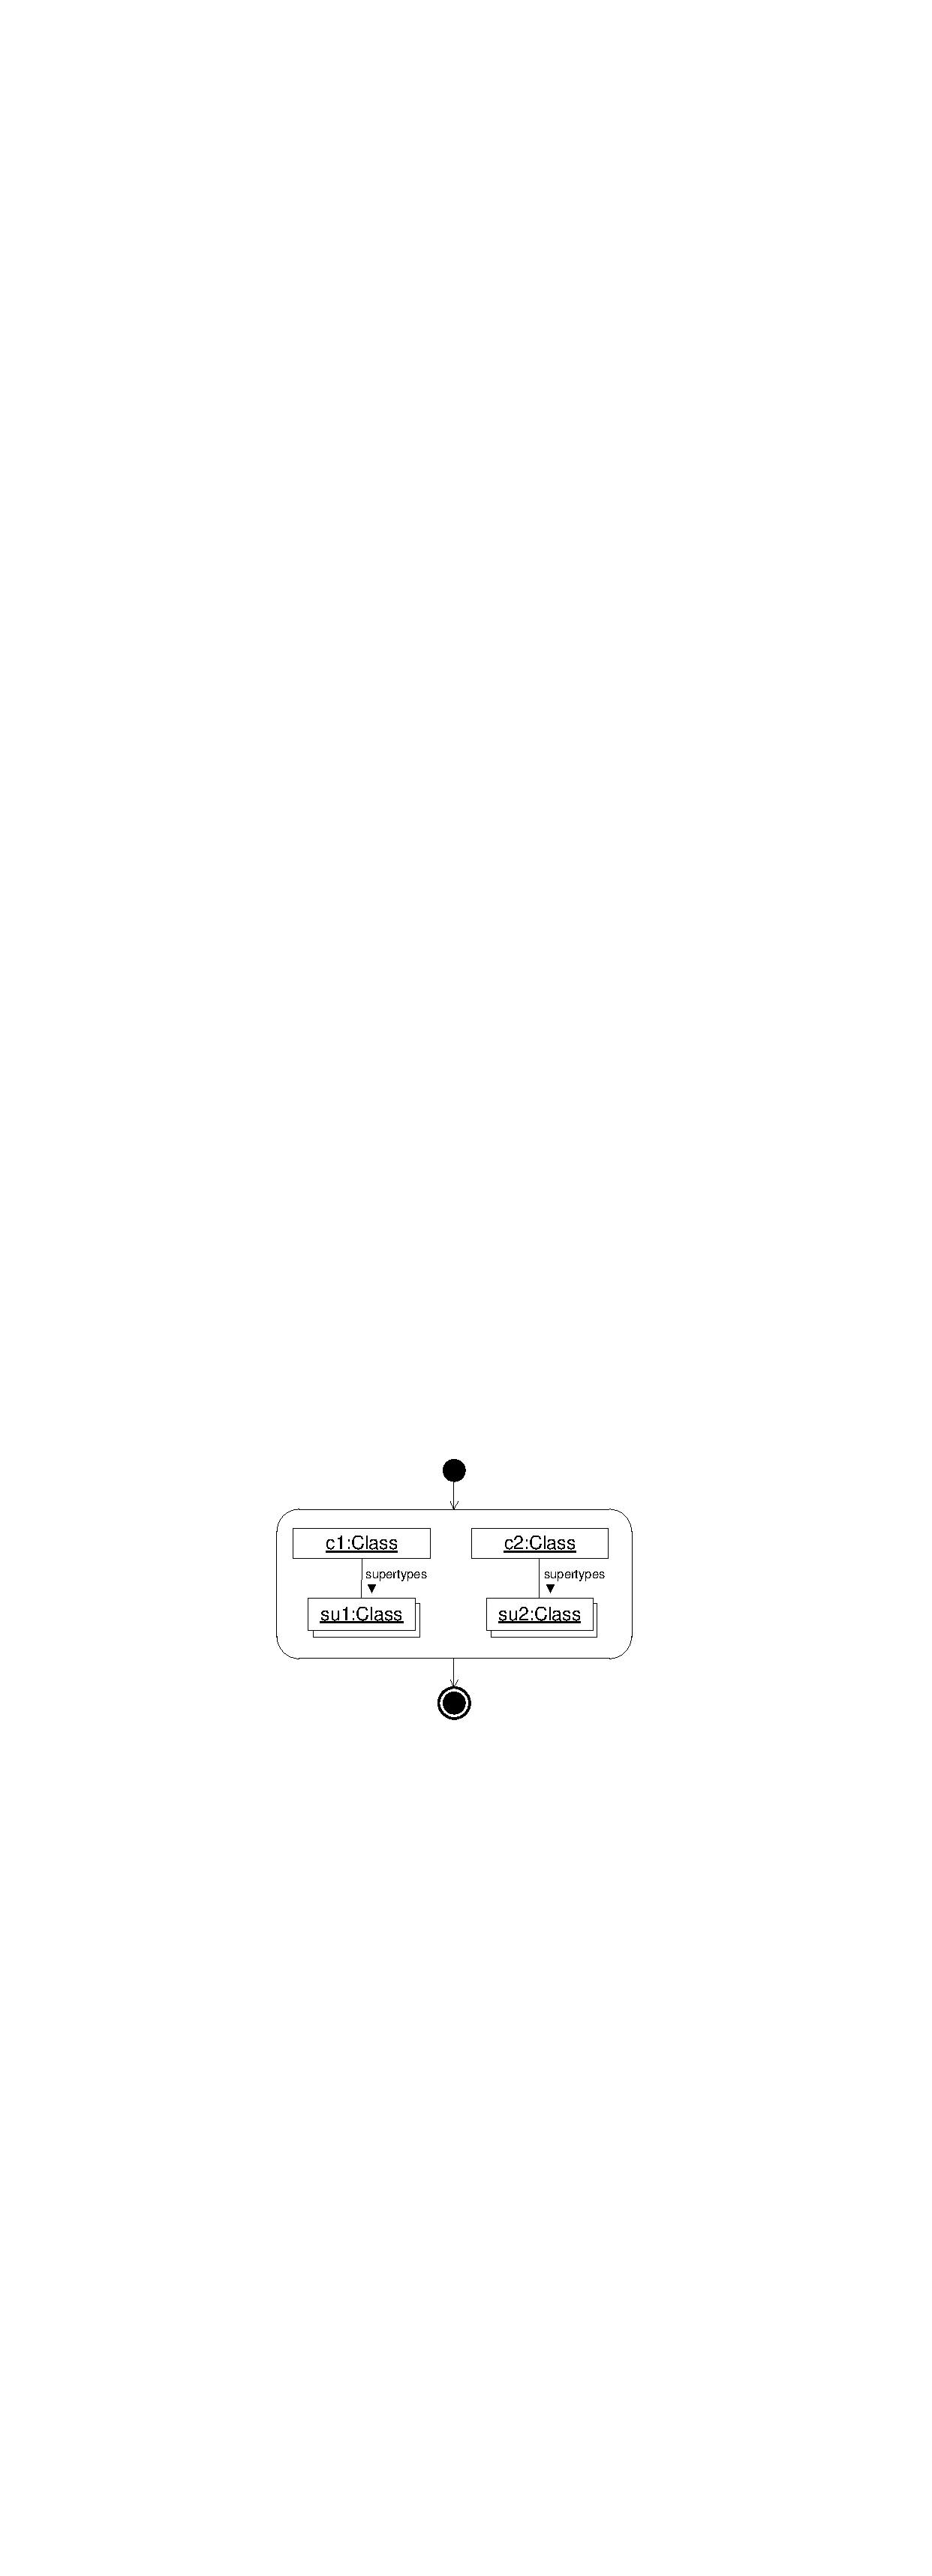
\includegraphics[scale=1.0]{figures/IsomorphismInObjectSets}
  \caption{Isomorphism in Object Sets}
  \label{fig:isoObjSet}
\end{figure}


\subsection{Special Link Kinds [CH]}

\subsubsection{Containment Relations [CH]}

\todoch{What is the semantics of a containment link? Current understanding: an element is contained in a container. What is the difference to to-many references which are containments?}

\todoch{Which classifiers are allowed for ContainerVariables? This should not only be the EMF collection types EList and EMap. Does a ContainmentLink need a reference as a type like normal LinkVariables?}

\subsubsection{Paths [MCP]}

\subsubsection{Link Constraints [CH]}

\todoch{What is the concrete Syntax for this?}

Link constraints are only applicable to link variables that reference an ordered to-many reference. 
\begin{itemize}
  \item FIRST = matches the first element in the list, requires one link variable
  \item LAST = matches the last element in the list, requires one link variable
  \item INDEX = matches the element at the specified index, requires one link variable
  \item DIRECT\_SUCCESSOR = requires two link variables, target of the second one must be located directly after the target of the first one in the list
  \item INDIRECT\_SUCCESSOR = requires two link variables, target of the second one must be located somewhere after the target of the first one in the list
\end{itemize}

\todoch{Is this semantic description correct/complete?}

\subsubsection{Maybe Links}

Disables the isomorphism check for two object variables, these two object variables may be matched to the same object.

\todoch{What is the concrete Syntax? Using a special pattern constraint as proposed in Alberts Habil is very low-level. Alternative version is proposed in Figure \ref{fig:maybeLink}.}

\begin{figure}[htbp]
  \centering
  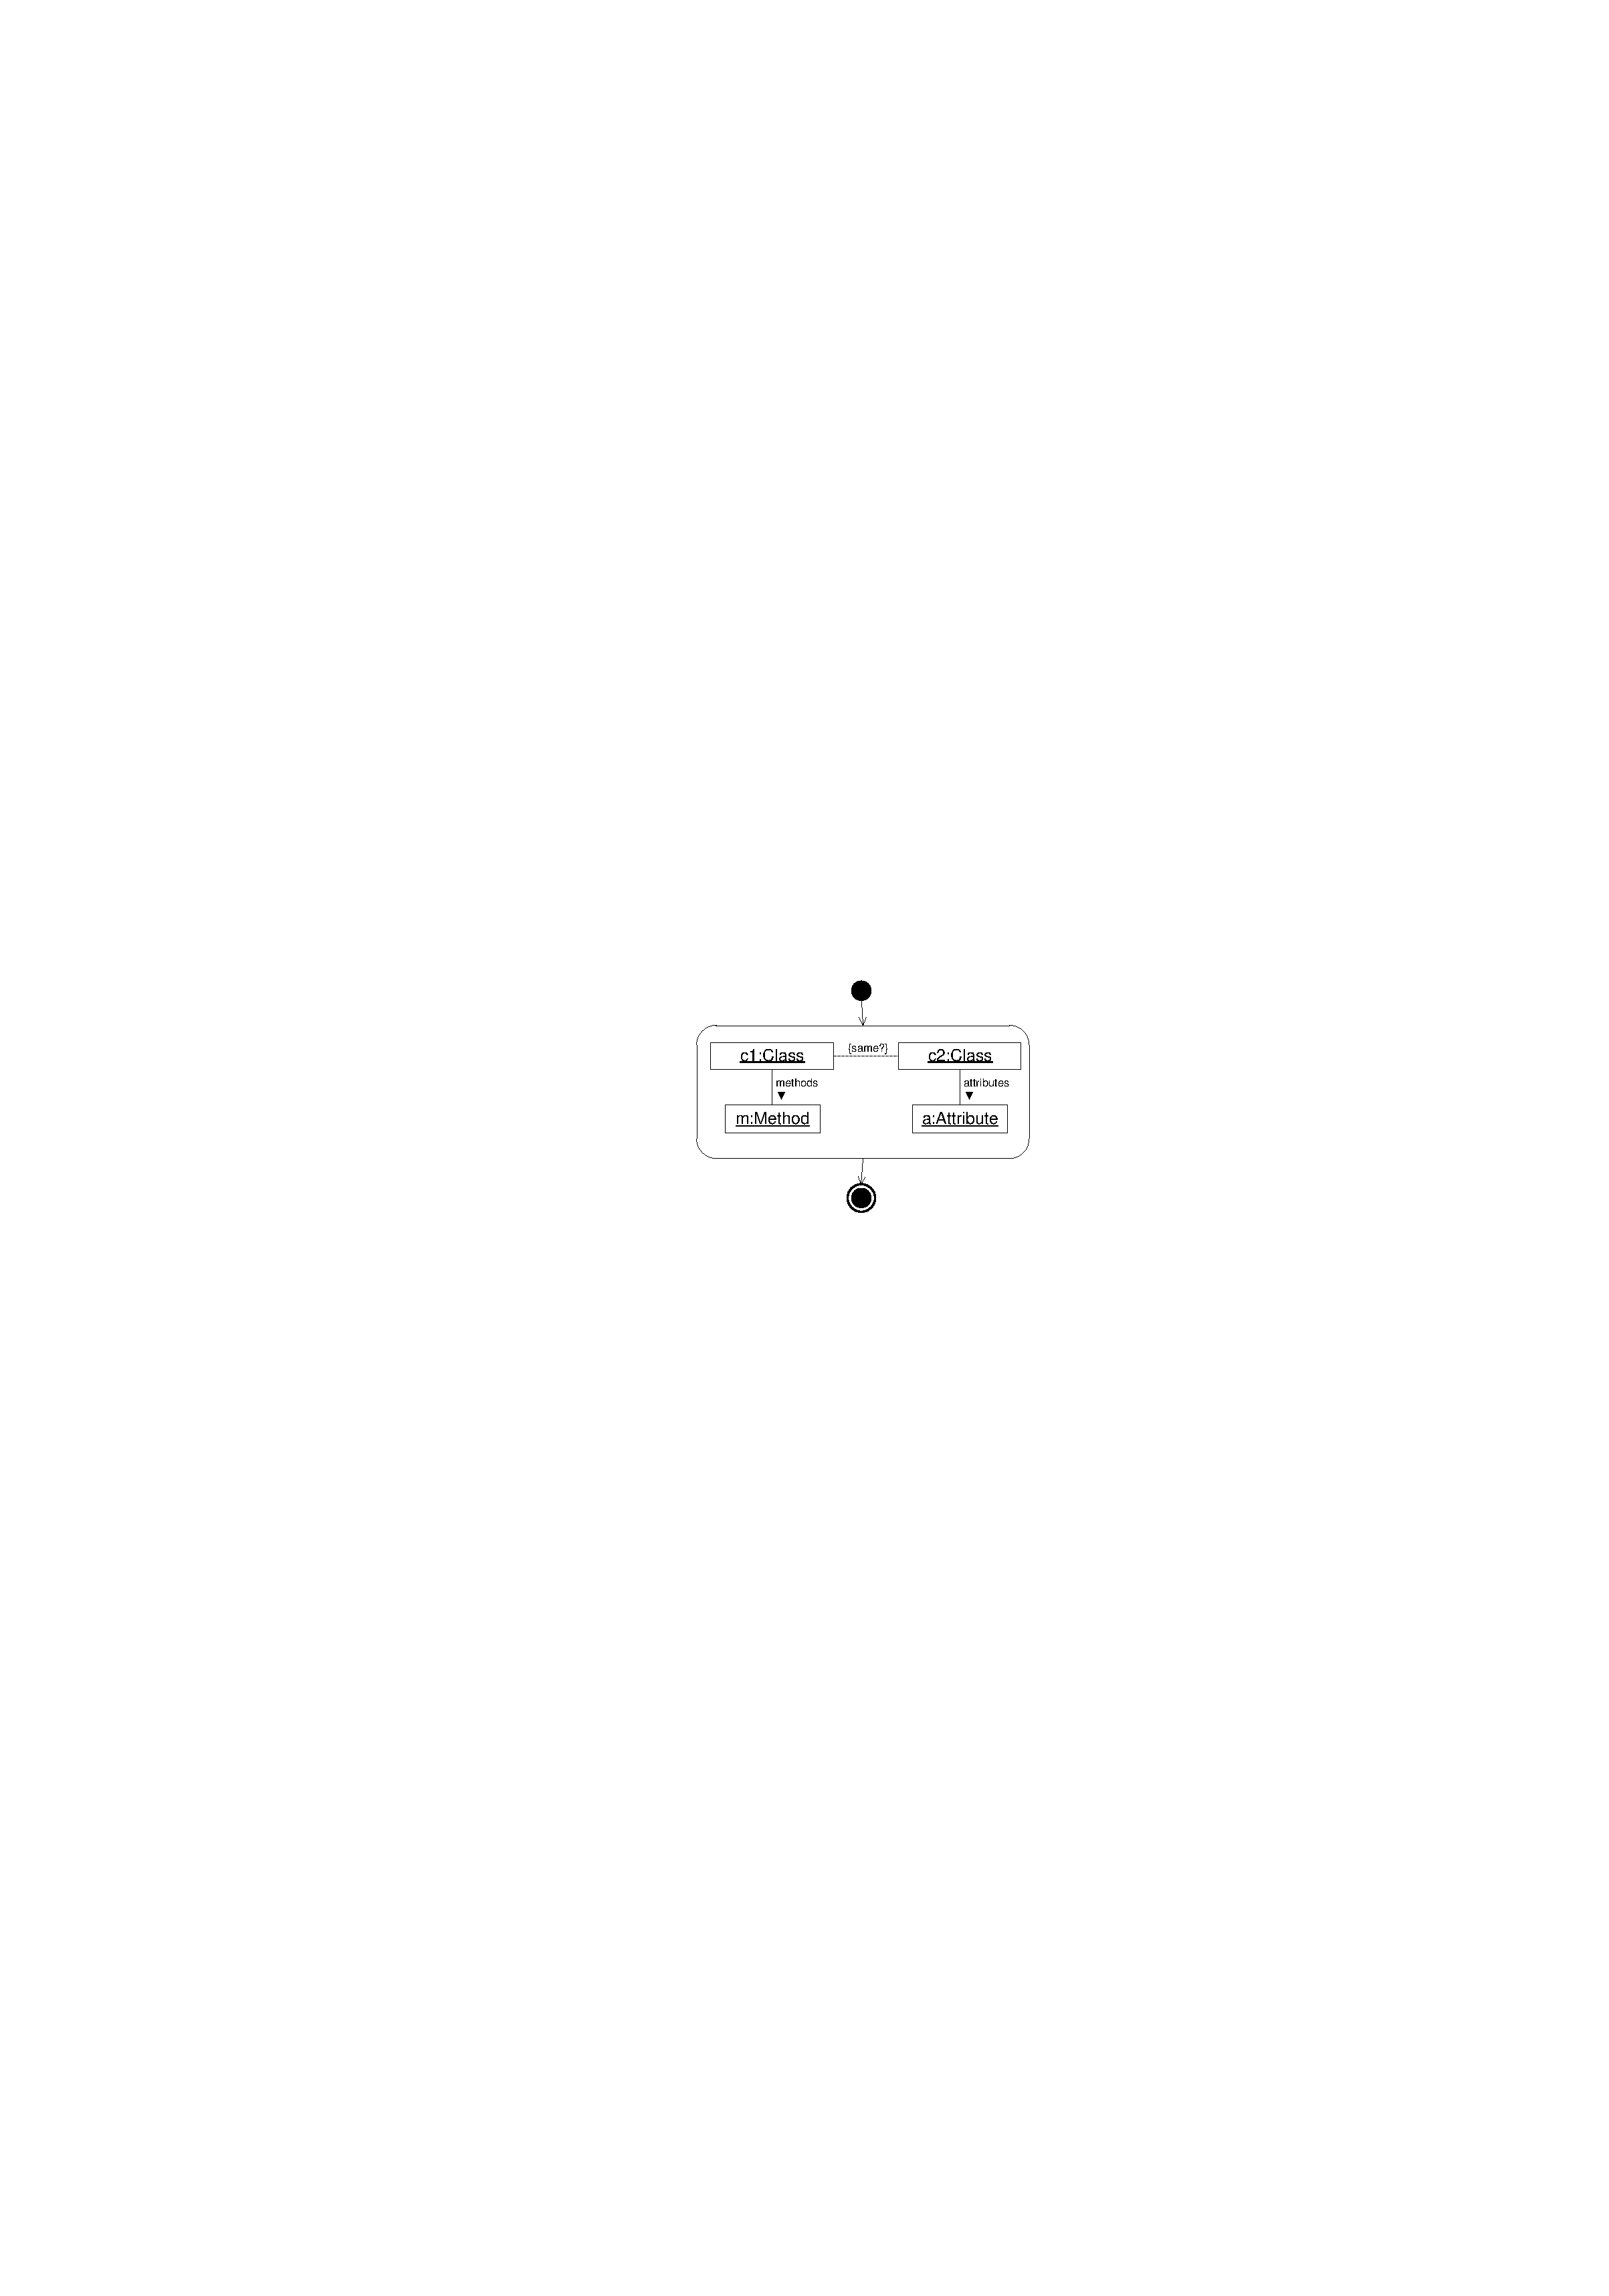
\includegraphics[scale=1.5]{figures/MaybeLink}
  \caption{Maybe Link}
  \label{fig:maybeLink}
\end{figure}

\subsection{Pattern Constraints [CH]}

\todoch{What happens when a pattern constraint is placed inside a for each story pattern (not inside a node in that pattern)? Proposal: The particular match must fulfill the pattern constraint, if it does not fulfill the pattern constraint, the match is rejected and the iteration continues.}

\subsection{Contained Pattern [MCP]}

patterns contained in other patterns, negative, semantics? review enhanced story patterns from Diss Florian Klein

\todomcp{Should contained pattern be marked as forEach? Idea for semantics: first the part of the pattern outside the forEach pattern is matched, then the forEach subpattern is applied to any match that may be located, the variables bound in a forEach subpattern may not be used in subsequent activities}

\begin{figure}[htbp]
  \centering
  
\includegraphics[scale=1.0]{figures/ContainedPattern}
  \caption{Different Kinds of Contained Patterns}
  \label{fig:containedPattern}
\end{figure}

\todomcp{Should contained pattern be marked as optional? Is currently possible in the meta-model. Idea for semantics: Whole pattern must be found, if found, variables may be used in subsequent activities, if pattern may not be found as a whole, matching still succeeds but all variables in the subpattern are not bound in subsequent activities.}

\todomcp{How deep may patterns be nested? What is the semantics of alternating binding semantics of sub-patterns, e.g. negative in optional in negative and so on.}

\subsection*{Old stuff from rejected paper}

Story patterns describe graph replacement rules that can be embedded into the activities of a story diagram. They are based on labeled, attributed graphs that are extended by a type model \cite{FNTZ00}. 
The types and references that are specified in the type model are used to type the nodes and edges within the story pattern.
Type models for story diagrams can be created, e.g., by using EMF Ecore \cite{SBP+08}.
In our example, we will use the meta-models shown in Figures~\ref{fig:sourceMetamodel} and~\ref{fig:targetMetamodel} as type models. The type model supports inheritance and polymorphism, i.e., a node of type \fe{Classifier} matches objects of types \fe{Classifier}, \fe{Class}, and \fe{PrimitiveType}.
This allows specifying graph replacement rules for object-oriented models.

In order to provide a concise notation, story patterns apply a short-hand notation depicting left-hand side and right-hand side in one graph. Nodes and edges being created (or deleted) are annotated with \small \verb|<<create>>| \normalsize (or  {\small \verb|<<destroy>>|\normalsize}, respectively). The matching of story patterns in a host graph requires an isomorphic matching of the pattern's left-hand side in the host graph, i.e., two nodes of the pattern may not be matched to the same node in the host graph \cite{FNTZ00,Roz97}. The matching is performed with respect to the types of the type model. The deletion of nodes is applied according to the Single Pushout Approach (SPO, \cite{Roz97}), i.e., dangling edges resulting from the deletion of nodes are deleted as well.

Figure~\ref{fig:SP} shows an example of a story pattern that simply adds a class to the set of classifiers of the source system (cf. Figure~\ref{fig:sourceMetamodel}).

\begin{figure}[htbp]
\begin{center}
  
\includegraphics[width=0.25\textwidth]{figures/StoryPattern}
  \caption{Simple story pattern}
  \label{fig:SP}
\end{center}
\end{figure}